% !TeX program = xelatex
% TeXora 主页截图用示例: 演示模式 (Shift+F5)
\documentclass[aspectratio=169]{ctexbeamer}
\usetheme{default}
\usefonttheme{professionalfonts}
\setbeamertemplate{navigation symbols}{}
\setbeamertemplate{footline}[frame number]
\setbeamercolor{frametitle}{fg=black}
\setbeamercolor{structure}{fg=cyan!45!black}
\usepackage{amsmath,amssymb,mathtools,booktabs,tikz}
\DeclarePairedDelimiter{\norm}{\lVert}{\rVert}
\DeclarePairedDelimiter{\abs}{\lvert}{\rvert}
\DeclarePairedDelimiter{\inner}{\langle}{\rangle}
\newcommand{\C}{\mathbb{C}}

\title{紧算子的谱理论及其数值逼近}
\subtitle{讨论班报告}
\author{TeXora 示例项目}
\date{2026 年 11 月}

\begin{document}

\begin{frame}
  \titlepage
\end{frame}

\begin{frame}{问题}
  \begin{itemize}
    \item 有限维: $\sigma(A)$ 即特征值全体, 至多 $n$ 个点.
    \item 无穷维有界算子: 谱可以是连续统, 也可以没有特征值.
    \item 紧算子介于二者之间: 谱的结构与矩阵十分接近.
  \end{itemize}
  \bigskip
  \centering
  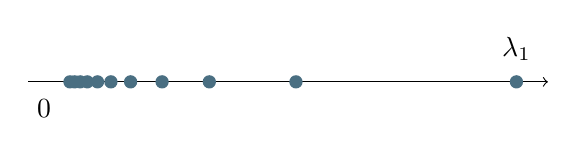
\begin{tikzpicture}[x=1cm,y=1cm]
    \draw[->] (-0.2,0) -- (6.4,0);
    \foreach \x in {6,3.2,2.1,1.5,1.1,0.85,0.68,0.55,0.46,0.39,0.33}
      \fill[cyan!45!black] (\x,0) circle (2.4pt);
    \node[below] at (0,-0.1) {$0$};
    \node[above] at (6,0.15) {$\lambda_1$};
  \end{tikzpicture}
\end{frame}

\begin{frame}{Riesz--Schauder 定理}
  \begin{block}{定理}
    设 $X$ 为无穷维 Banach 空间, $T$ 为 $X$ 上的紧算子, 则
    \begin{enumerate}
      \item $0\in\sigma(T)$;
      \item $\sigma(T)\setminus\{0\}$ 中每一点都是重数有限的特征值;
      \item $\sigma(T)$ 至多可数, 且除 $0$ 外无其他聚点.
    \end{enumerate}
  \end{block}
  \pause
  证明要点: Riesz 引理 + 紧性 $\Rightarrow$ 不存在两两远离的特征向量列.
\end{frame}

\begin{frame}{紧自伴算子的谱定理}
  设 $T$ 为 Hilbert 空间 $H$ 上的紧自伴算子, 则
  \begin{equation*}
    Tx=\sum_{n\ge1}\lambda_n\inner{x,e_n}e_n,\qquad \abs{\lambda_1}\ge\abs{\lambda_2}\ge\cdots\to0 .
  \end{equation*}
  \pause
  若 $T\ge0$, 则有极小极大刻画
  \begin{equation*}
    \lambda_n=\min_{\dim V=n-1}\ \max_{x\perp V,\ \norm{x}=1}\inner{Tx,x}.
  \end{equation*}
\end{frame}

\begin{frame}{例: 核 $\min\{s,t\}$}
  \begin{equation*}
    (Tf)(s)=\int_0^1\min\{s,t\}f(t)\,\mathrm{d}t,\qquad
    \lambda_n=\frac{1}{(n-\frac12)^2\pi^2}.
  \end{equation*}
  \centering
  \begin{tabular}{cccc}
    \toprule
    $n$ & 精确值 & $N=50$ & $N=200$ \\
    \midrule
    1 & 0.405285 & 0.405318 & 0.405287 \\
    2 & 0.045032 & 0.045065 & 0.045034 \\
    3 & 0.016211 & 0.016245 & 0.016213 \\
    \bottomrule
  \end{tabular}
\end{frame}

\begin{frame}{误差阶}
  \begin{itemize}
    \item 中点求积: 网格加密 4 倍, 相对误差约为原来的 $1/16$.
    \item 与 $O(N^{-2})$ 的理论阶一致.
    \item 高阶特征值误差更大: 特征函数振荡更快.
  \end{itemize}
\end{frame}

\begin{frame}{小结}
  \begin{enumerate}
    \item 紧算子的非零谱只含有限重特征值, 唯一可能的聚点是 $0$.
    \item 紧自伴算子可以像对称矩阵一样对角化.
    \item Nyström 离散化给出二阶收敛的特征值逼近.
  \end{enumerate}
  \bigskip
  \centering\Large 谢谢!
\end{frame}

\end{document}
